\apendice{Plan de Proyecto Software}

\section{Introducción}
La planificación es una parte importante de un proyecto. En esta parte se estima el trabajo, el tiempo y el dinero necesario para realizar el proyecto. Hay que analizar todas las partes que forman el proyecto, con esto sabemos los recursos que necesitaremos. Podemos dividir la planificación en planificación temporal y estudio de la viabilidad.
\begin{itemize}
\item Planificación temporal: Se elabora un calendario en el que se estima el tiempo que tardaremos en realizar cada una de las tareas del proyecto. 
\item Estudio de viabilidad: Si el proyecto es viable o no. Podemos dividirlo en dos:
\begin{itemize}
\item Viabilidad económica: Se calculan los beneficios y costes del proyecto.
\item Viabilidad legal: Hay que ver si cumple todas las leyes, y en el software que tiene las licencias y la ley de protección de datos.
\end{itemize}
\end{itemize}

\section{Planificación temporal}
Para la planificación del proyecto hemos utilizado la metodología Scrum, aunque esta metodología está pensaba para trabajar en equipo, consiste en realizar unas entregas parciales y regulares del producto final, es recomendable para proyectos en entornos complejos, donde se necesitan obtener resultados pronto, y la innovación, la competitividad, la flexibilidad y la productividad son fundamentales.
En nuestro caso a través de GitHub:
\begin{itemize}
\item Creamos un Milestone correspondiente a la semana que estamos.
\item Creamos las tareas que realizaremos esa semana habladas en la reunión semanal.
\item Para gestionar el tiempo de las tareas utilizaremos ZenHub, que es una herramienta que incluye el  navegador.
\item Según vamos realizando las tareas las vamos cerrando, y así podremos observar el gráfico que nos muestra en \textit{burndown chart}, en el que podremos ver el progreso.
\end{itemize}
A continuación se analizan y detallan las tareas realizadas en todos los sprints que se han realizado.
\subsection{Sprint 0 (18/09/17 - 25/09/17)}
En la reunión para planificar este sprint es cuando comenzó el proyecto. En ella se concreta por encima en que consiste el problema que vamos a llevar a cabo.
En esta primera semana, se ha dedicado a la documentación de las herramientas que se van a usar y de distintos artículos, las tareas son:
\begin{itemize}
\item Refrescar los conocimientos de GitHub.
\item Documentación sobre \LaTeX~\cite{wiki:latex}, y su posterior instalación y configuración.
\item Leer artículo Disturbing Neighbors~\cite{disturbingneighbors}.
\item Documentación sobre Bagging~\cite{scikitlearn}.
\end{itemize}

Esta semana se han cumplido todas las tareas, aunque como todavía no sabía utilizar correctamente GitHub, no creé bien el Milestone por lo que esta semana no tenemos burndown.

\subsection{Sprint 1 (26/09/17 - 02/10/17)}
Esta semana, se ha dedicado a la documentación del funcionamiento de bagging y empezar con el primer clasificador Disturbing Neighbors, las tareas son:
\begin{itemize}
\item Reducir el conjunto de datos. Reducimos el conjunto de datos para quedarnos sólo con los datos que valoraremos para entrenar, estos datos se eligen mediante un subespacio aleatorio (un array aleatorio de 0 y 1).
\item Calculamos las distancias al vecino más cercano para ello en nuestro caso utilizaremos la distancia de euclides. Los vecinos sobre los que calculamos dichas distancias son unas instancias del conjunto elegidas al azar. 
\item Funcionamiento del BaggingClassifier. Como nosotros también vamos a hacer un clasificador, entender como se usa el fit, predict y precict\_proba.
\item Entrenamiento. Entrenamos los datos mediante el método \texttt{fit} que tenemos que programar.
\item Crear la clase Disturbing Neighbors. Es la clase en la que programaremos nuestro clasificador.
\end{itemize}

Esta semana se han cumplido todas las tareas.

\subsection{Sprint 2 (02/10/17 - 10/10/17)}
Esta semana, se ha dedicado a la corrección de errores de la semana pasada y a seguir avanzando con la clase, las tareas son:
\begin{itemize}
\item Corregir errores. En la reunión los tutores vieron algunos fallos que hay que corregir del método \texttt{fit}, en el que entrenamos nuestro conjunto de datos.
\item Función \texttt{predict}. Empezamos con el siguiente método de la clase, en el que después de haber entrenado los datos ahora podemos predecir con ellos.
\item Mostrar árbol de decisión. Como hemos entrenado nuestros datos podemos mostrar gráficamente los resultados para que sean más apreciables.
\item Estructurar bien el código. Esto lo hacemos para que en un futuro sea más fácil trabajar.
\end{itemize}

Esta semana se han cumplido todas las tareas, esta semana terminé de entender como utilizar bien Github, por lo que no creé bien el Milestone por lo que esta semana no tenemos burndown.

\subsection{Sprint 3 (10/10/17 - 15/10/17)}
Esta semana, se ha dedicado a la corrección de errores de la semana pasada y a mostrar los resultados en un notebook, las tareas son:
\begin{itemize}
\item Corregir errores. La clase no funciona correctamente, ya que algunos de los métodos no hace lo que tienen que hacer, esta tarea no la conseguiremos acabar esta semana, tendremos que dedicar tiempo la próxima semana.
\item Mostrar árbol en un notebook. Una vez conseguido que la primera versión del clasificador funcione correctamente, mostraremos un árbol de decisión en un notebook para poder observar mejor los resultados.
\end{itemize}

Esta semana se han cumplido todas las tareas, aunque una de las tareas estaba particionada entre esa semana y la siguiente.

En la figura~\ref{fig:Milestone4} se muestra el gráfico del Sprint 3.

\begin{figure}
\centering
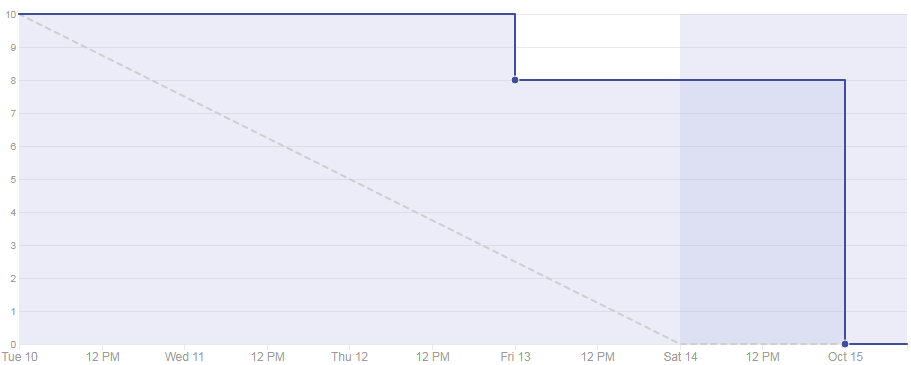
\includegraphics[width=0.95\textwidth]{Milestone4}
\caption{Burndown del sprint 3}
\label{fig:Milestone4}
\end{figure}

\subsection{Sprint 4 (17/10/17 - 23/10/17)}
Esta semana, se ha dedicado a corregir algún error más, a comentar el código y añadir algún nuevo método para que el clasificador funcione mejor:
\begin{itemize}
\item Comentar los métodos. Comentamos los diferentes métodos según el formato de Python~\cite{comment}.
\item Semilla. Creamos una semilla, esto lo hacemos para inicializar los valores aleatorios y así conseguir que siempre empiece por el mismo, esto lo hacemos para cuando hacemos pruebas siempre las haga con los mismos datos.
\item Vecinos molestones. No están calculados correctamente.
\item Corregir fallos. Sigue dándome algún fallo, no hace lo que debería.
\item Método \texttt{calculate\_features}. Creamos un método en el que si recibe un numero menor de 1, es el porcentaje de las características con las que nos quedaremos, mientras que si lo que recibe es un número mayor de 1 es un número entero, que índica el valor exacto de las características que escogemos.
\end{itemize}

Esta semana se han cumplido todas las tareas, terminamos de corregir los fallos, aunque posteriormente iremos mejorando el clasificador.

En la figura~\ref{fig:Milestone5} se muestra el gráfico del Sprint 4.

\begin{figure}
\centering
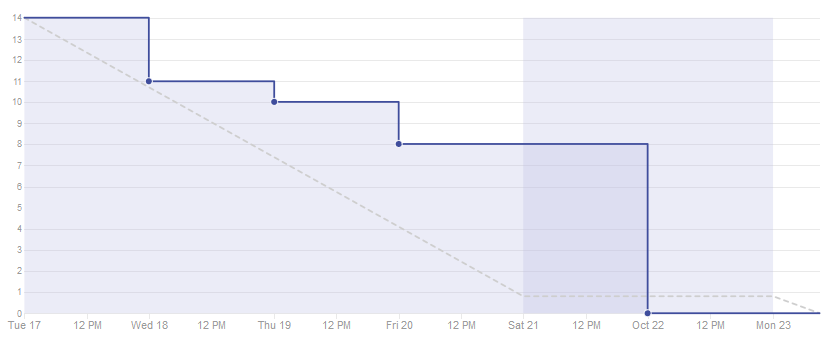
\includegraphics[width=0.95\textwidth]{Milestone5}
\caption{Burndown del sprint 4}
\label{fig:Milestone5}
\end{figure}

\subsection{Sprint 5 (24/10/17 - 30/10/17)}
Esta semana, se ha dedicado mayormente a empezar a documentar en la memoria, a parte de alguna otra tarea:
\begin{itemize}
\item Semilla. No estaba hecha correctamente, hay que hacer alguna modificación.
\item Subir estructura de proyecto a GitHub. Organizamos y estructuramos bien la estructura del proyecto en GitHub.
\item Partición de entrenamiento. Dividimos el conjunto de entrenamiento para pasar una parte al fit y otra parte al predict.
\item Memoria: Introducción. Sobre que va ir nuestro proyecto, una breve explicación.
\item Memoria: Objetivos del proyecto. Los objetivos que cumpliremos en el proyecto.
\item Memoria: Conceptos teóricos. Los conceptos necesarios para poder entender y trabajar en el proyecto.
\item Anexo: Manual del programador. La información que necesitara un programador que quiera seguir con el proyecto.
\item Anexo: Manual del usuario. Información que necesitará un usuario para poder usar las funcionalidad del proyecto.
\end{itemize}

Esta semana no se han cumplido todas las tareas, las partes del anexo de manual de programador y usuario no han podido llegar a realizar, aunque en el burndown muestre que están realizadas no es así.

En la figura~\ref{fig:Milestone6} se muestra el gráfico del Sprint 5.

\begin{figure}
\centering
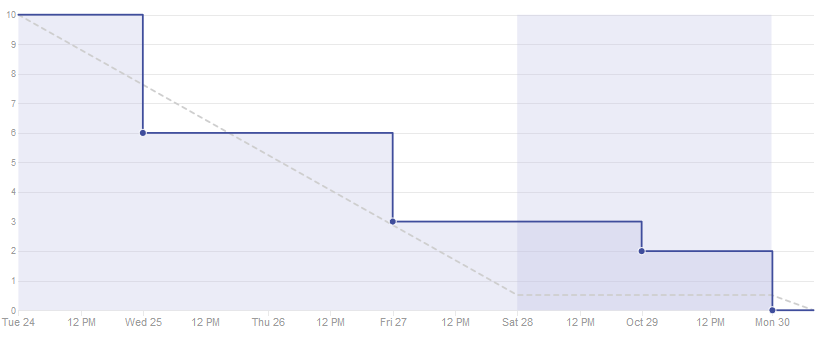
\includegraphics[width=0.95\textwidth]{Milestone6}
\caption{Burndown del sprint 5}
\label{fig:Milestone6}
\end{figure}

\subsection{Sprint 6 (31/10/17 - 05/11/17)}
Esta semana, se ha dedicado mayormente a empezar a documentar en la memoria, a parte de alguna otra tarea:
\begin{itemize}
\item Clase funcional. Hacemos la clase funcional, como puede ser cambiar los for por map, para que luego se más rápido en la ejecución.
\item Probar clase en Spyder. Para ver que todo la clase funciona correctamente la probamos.
\item Función predecir probabilidades. Creamos un nuevo método llamado \texttt{predict\_proba} que nos devolverá las probabilidades.
\item Memoria: Técnicas y herramientas. Añadiremos técnicas y herramientas necesarias para entender y poder trabajar con el proyecto.
\item Método \texttt{train\_test\_split}: Usaremos el método para dividir nuestro conjunto de datos, dicho método es más eficaz que como lo estábamos haciendo la semana pasada.
\item Correcciones de estilo y mejoras al código DN: Cambiaremos algunas variables a privadas, los comentarios los ponemos en inglés, y utilizaremos el chequeador de sintaxis \url{http://pep8online.com/} para tener un estilo adecuado.
\end{itemize}

Esta semana se han cumplido todas las tareas, al probar la clase en spyder ha dado algunos errores, sobre todo al importar la clase DisturbingNeihgbors, y algunos errores menores.

En la figura~\ref{fig:Milestone7} se muestra el gráfico del Sprint 6.

\begin{figure}
\centering
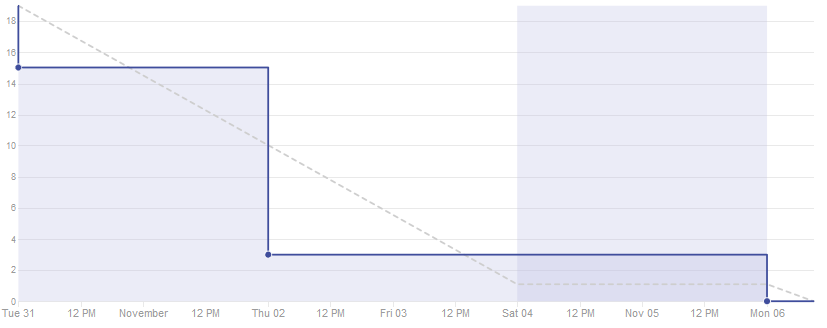
\includegraphics[width=0.95\textwidth]{Milestone7}
\caption{Burndown del sprint 6}
\label{fig:Milestone7}
\end{figure}

\subsection{Sprint 7 (07/11/17 - 20/11/17)}
Esta semana, se ha dedicado mayormente a empezar a documentar en la memoria, a parte de alguna otra tarea:
\begin{itemize}
\item Pasarle a bagging la clase DN. Probamos a pasarle a bagging nuestra clase Disturbing Neighbors. Como bagging no soporta múltiples salidas, para ello lo solucionaremos utilizando OneVsRestClassifier, esto permitirá que bagging soporte múltiples salidas.
\item Hacer funcional el método \texttt{nearest\_neighbor}. Conseguir que el método \texttt{nearest\_neighbor} funcione sin utilizar ningún bucle for.
\item Memoria Conceptos teóricos. Añadir nuevos conceptos teóricos como Multi-Label o ensemble.
\item Iteraciones sobre los métodos \texttt{fit}, \texttt{predict} y \texttt{predict\_proba}. Hasta ahora solo se ejecutaba una vez cada método, pero para que esto sea eficaz queremos que se ejecute un número de iteraciones. El \texttt{fit} será el más fácil solo hay que realizar ese método el número de iteraciones requeridas. Para poder calcular el \texttt{predict} tenemos que ir guardando los valores del fit y calcular el promedio. Por último el \texttt{predict\_proba} se calculará igual que el predict.
\item Estructurar notebook. Estructuramos el notebook de jupyter, para que sea más fácil de entender.
\item Método \texttt{cross validation}: Para crear los conjuntos de entrenamiento y test usar la validación cruzada.
\end{itemize}

Esta semana se han cumplido todas las tareas, aunque las tareas de hacer funcional el método \texttt{nearest\_neighbor} y \texttt{cross validation}, me han hecho dedicar más horas de las esperadas, en el primer caso por mi poco conocimiento sobre el uso de los mapas en python y en el segundo caso por los diversos errores que me salían al intentar compilar.

En la figura~\ref{fig:Milestone8} se muestra el gráfico del Sprint 7.

\begin{figure}
\centering
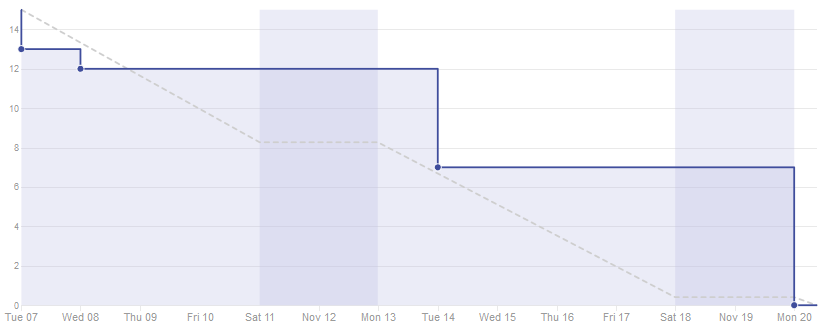
\includegraphics[width=0.95\textwidth]{Milestone8}
\caption{Burndown del sprint 7}
\label{fig:Milestone8}
\end{figure}

\subsection{Sprint 8 (21/11/17 - 27/11/17)}
Esta semana, se ha dedicado a terminar definitivamente el Disturbing Neighbors y documentarme sobre el siguiente algoritmo Random Oracles:
\begin{itemize}
\item Comentar Notebooks. Comentamos los notebooks, para ir explicando lo que realizamos en cada paso.
\item Estilo. Como hemos realizado alguna modificación volvemos a comprobar que el estilo es el correcto.
\item Excepciones. Ponemos excepciones para los casos que pueda ocurrir un error.
\item Artículo Random Oracles~\cite{randomoracles}. Documentación sobre el nuevo algoritmo Random Oracles.
\item Acabar \texttt{predict\_proba} y comentar nuevos métodos. Acabamos el \texttt{predict\_proba} para cuando hacemos iteraciones, y comentamos los nuevos métodos que hemos creado.
\item Método \texttt{score} iteraciones. Hacer correctamente el método \texttt{score} cuando hacemos iteraciones.
\end{itemize}

Esta semana una de las tareas no se ha acabado por lo que aparecerá en el Sprint 9, ninguna de las tareas ha llevado mas tiempo del estimado, ya que ninguna de las tareas ha dado muchos problemas.

En la figura~\ref{fig:Milestone9} se muestra el gráfico del Sprint 8.

\begin{figure}
\centering
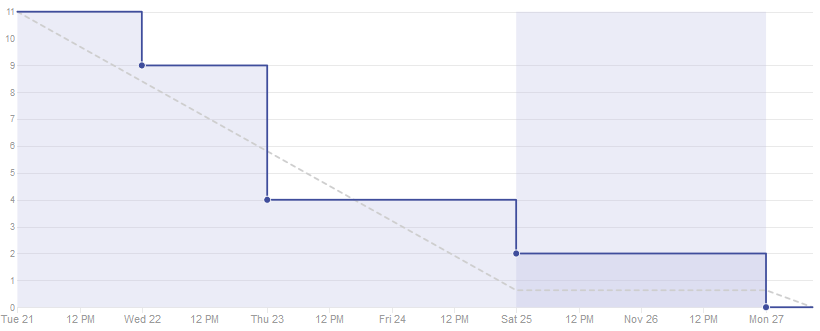
\includegraphics[width=0.95\textwidth]{Milestone9}
\caption{Burndown del sprint 8}
\label{fig:Milestone9}
\end{figure}

\subsection{Sprint 9 (28/11/17 - 04/12/17)}
Esta semana, se ha dedicado a probar unos datos reales en Disturbing Neighbors, a comenzar con el algoritmo Random Oracles y a otras tareas menores:
\begin{itemize}
\item Pasar un conjunto de datos reales a DN. Probamos el clasificador con un conjunto de datos reales, lo escogeremos de mulan o meka. Como el archivo es .arff, necesitaremos aprender como leer un archivo .arff en python.
\item Fit Random Oracles. Creamos el \texttt{fit} y los métodos necesarios para su funcionamiento.
\item Mejorar la descripción de las excepciones. Cambiamos la descripción de las excepciones para que no sean tan genéricas, y ayuden a entender al usuario el problema.
\item Revisar Ortografía. Revisar los comentarios y todo lo escrito hasta la fecha para ver que no hay faltas de ortografía.
\item Comentarios globales de los notebook. Poner comentarios encima de cada parte de código para que sea más entendible.
\end{itemize}

Esta semana se han cumplido todas las tareas menos la del predict del Random Oracles, las tareas de pasar un conjunto reales y el fit del random oracles, han llevado más tiempo del esperado, la primera por mi desconocimiento sobre los archivos arff, y la segunda porque no comprendí bien como debía funcionar el fit.

En la figura~\ref{fig:Milestone10} se muestra el gráfico del Sprint 9.

\begin{figure}
\centering
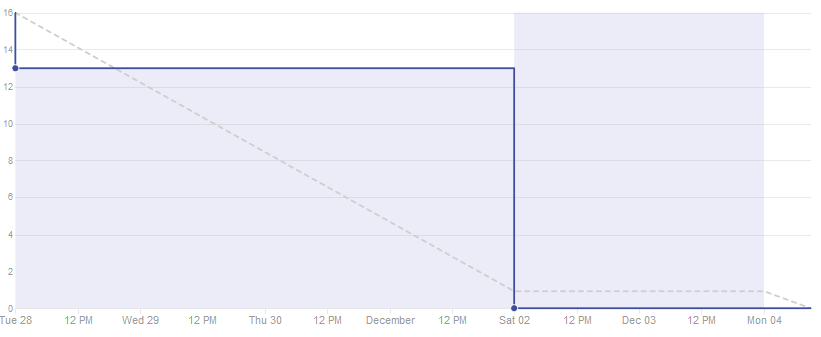
\includegraphics[width=0.95\textwidth]{Milestone10}
\caption{Burndown del sprint 9}
\label{fig:Milestone10}
\end{figure}

\subsection{Sprint 10 (05/12/17 - 11/12/17)}
Esta semana, se ha dedicado a dejar casi terminado el clasificador Random Oracles y a otras tareas menores:
\begin{itemize}
\item Predict Random Oracles. Realizamos el método \texttt{predict}.
\item Avanzar en la documentación. Empezar con la documentación, ya que está muy retrasada.
\item Mejorar método \texttt{fit}. Hacer funcional el código y si se puede reducirlo.
\item Método \texttt{predict\_proba}. Realizamos el método \texttt{predict\_proba}.
\item Iteraciones clase Random Oracle. Como en Disturbing Neighbors tenemos que hacer iteraciones sobre la clase Random Oracles.
\item Revisión de código. Cambiar el nombre de algunas variables o funciones para que su significado tenga que ver con el nombre.
\item Notebooks para el clasificador Random Oracle. Hacer notebooks para el clasificador Random Oracle, uno sin iteraciones, otro con iteraciones y otro con datos reales.
\end{itemize}

Esta semana se han cumplido todas las tareas, ninguna de las tareas ha dado muchos problemas a la hora de llevarla a cabo.

En la figura~\ref{fig:Milestone11} se muestra el gráfico del Sprint 10.

\begin{figure}
\centering
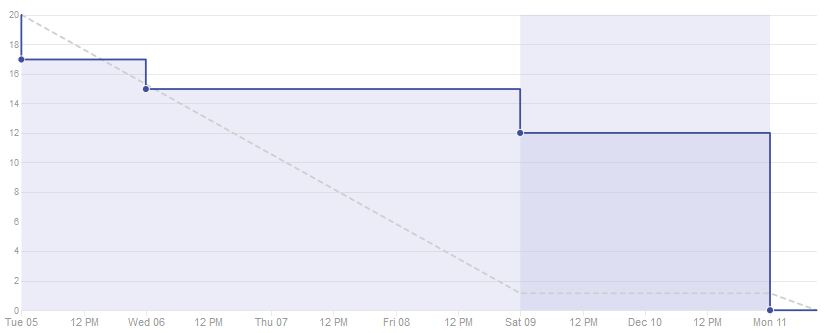
\includegraphics[width=0.95\textwidth]{Milestone11}
\caption{Burndown del sprint 10}
\label{fig:Milestone11}
\end{figure}

\subsection{Sprint 11 (12/12/17 - 18/12/17)}
Esta semana, se ha termina algunos detalles del Random Oracles, y se se ha empezado con el siguiente clasificador Random Forest:
\begin{itemize}
\item Artículo Rotation Forest~\cite{rotationforest}. Leer el artículo Rotation Forest, para entender el nuevo algoritmo que vamos realizar.
\item Notebooks. Mejorar los notebooks, creando una función que según un parámetro nos llame al clasificador Disturbing Neighbors o al Random Oracles.
\item Herencia. Usar la herencia, ya que una de las clases llamada \texttt{homogeneous\_ensembles} , es la que hace las iteraciones, y sus herederos serían las clases de Disturbing Neighbours y Random Oracles.
\item Rotation Forest dividir. Dividimos el conjunto de datos ($X$) en grupos de 3, usamos permutaciones para evitar repetidos.
\item Rotation Forest PCA. Cuando ya tenemos los grupos, usaremos \texttt{PCA} sobre cada uno de los grupos, en los que haremos primero fit y luego transform.
\item Rotation Forest fit. Volvemos a juntar los grupos en uno solo, y sobre este nuevo conjunto de datos ($X'$) hacemos el \texttt{fit}.
\item Correcto estilo Random Oracles. Utilizamos el chequeador de sintaxis de PEP8 online para que es el estilo que estamos siguiendo \url{http://pep8online.com/}.
\item Error encontrado en RO en el método \texttt{predict\_proba}. Encontramos un error cuando realizamos iteraciones sobre el método \texttt{predict\_proba} de la clase Random Oracles, ya que como lo probamos con un árbol cuando en una de las iteraciones si tiene el mismo labelset devuelve una predicción con tamaño uno, por lo tanto para corregir esto lo que hacemos es calcular las probabilidades con el método \texttt{predict}, ya que este sí funciona correctamente.
\item Comentar correctamente las clases. Algunos comentarios están incompletos y algunos métodos les falta comentarios.
\item Compactar los notebooks. Al final tener 3 notebooks en total, uno sin iteraciones, otro con iteraciones y otro con datos reales. Para diferenciar que clasificador queremos utilizar, instanciamos cada clasificador en una celda distinta, y después ejecutamos la celda del clasificador que queremos usar.
\item Avanzar con la Memoria. Esta semana avanzaré en la parte de planificación temporal, añadimos algunos sprint.
\end{itemize}

Esta semana se han cumplido todas las tareas, el error encontrado en el método \texttt{predict\_proba} me ha llevado mucho tiempo corregirlo, por lo que en la memoria no pude dedicarle todo el tiempo que quería.

En la figura~\ref{fig:Milestone12} se muestra el gráfico del Sprint 11.

\begin{figure}
\centering
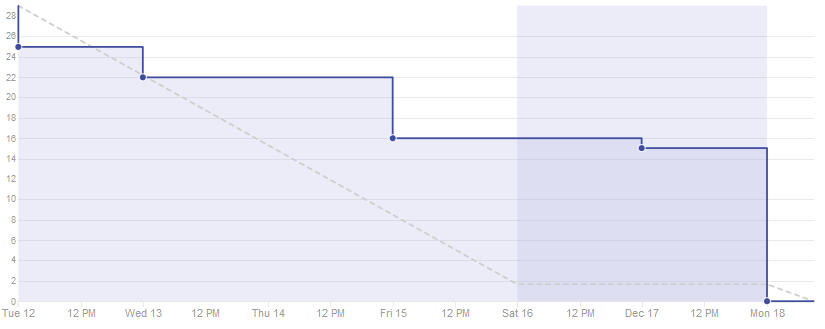
\includegraphics[width=0.95\textwidth]{Milestone12}
\caption{Burndown del sprint 11}
\label{fig:Milestone12}
\end{figure}

\subsection{Sprint 12 (19/12/17 - 25/12/17)}
Esta semana, se ha dedicado a avanzar con el algoritmo Rotation Forest y se añadir herencias a los algoritmos creados anteriormente:
\begin{itemize}
\item \texttt{predict} RF. Programar el método \texttt{predict} de Rotation Forest.
\item \texttt{predict\_proba} RF. Programar el método \texttt{predict\_proba} de Rotation Forest.
\item Añadir a la herencia de DN y RO. Con la clase ya acabada ahora la añadiremos la herencia, dicha herencia es sobre \texttt{homogeneous\_ensembles} y agregación sobre Rotation Forest.
\item Notebook RF. Añadir a los notebooks creados el clasificador Rotation Forest, y ver que funciona correctamente.
\item Seleccionar una muestra RF. Seleccionamos un muestra de cada uno de los subgrupos, por defecto el tamaño de dicha muestra será del 75\% de los datos. Dicha muestra la usaremos para entrenar pero para transformar le pasaremos el subgrupo entero.
\item Seleccionar una instancias en base a las clases. Lo primero elegimos las distintas clases($y$), después elegimos aleatoriamente una muestra de esas las distintas clases, y por último seleccionamos del conjunto de datos($X$) las instancias correspondientes a la muestra de esas clases.
\item Evitar código duplicado en los notebooks. La creación del conjunto de datos, la asignación de la semilla y la división del conjunto de datos en entrenamiento y test deben estar una única vez, y no repetidas en cada casilla de cada clasificador.
\end{itemize}

Esta semana se han cumplido todas las tareas, el tiempo empleado ha sido el previsto, ya que ninguna de las tareas ha dado demasiados problemas.

En la figura~\ref{fig:Milestone13} se muestra el gráfico del Sprint 12.

\begin{figure}
\centering
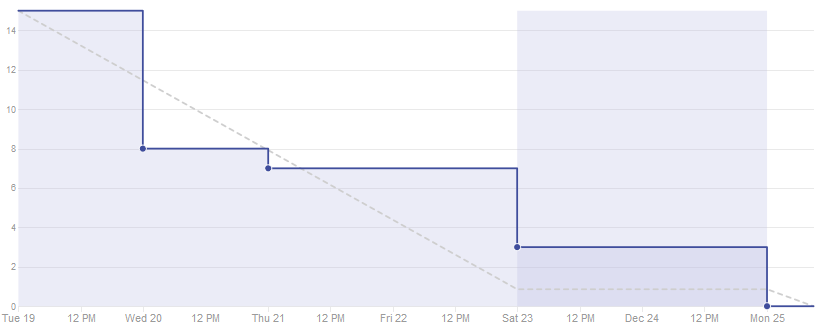
\includegraphics[width=0.95\textwidth]{Milestone13}
\caption{Burndown del sprint 12}
\label{fig:Milestone13}
\end{figure}

\subsection{Sprint 13 (26/12/17 - 07/01/18)}
Esta semana, se han tratado diversas temas, entre ellos, referencias en la documentación, dibujar gráficas para los clasificadores base, o que los algoritmos creados funciones también para Single-Label:
\begin{itemize}
\item Incluir referencias en la documentación. Añadimos referencias en la memoria y el anexo.
\item Funcional RF. Hacemos funcional el método \texttt{fit} de Rotation Forest.
\item Código repetido RF. Crear funciones para evitar el código repetido en Rotation Forest.
\item Memoria. Añadir los sprint que faltan.
\item Buscar información gráficas. Buscar información en otros Multi-Label de scikit learn para ver como dibujan los gráficos, que muestren los datos y como se dividen.
\item Dibujar gráficas. Dibujamos las gráficas de cada uno de los algoritmos (DN, RO, RF), para ver como se divide el conjunto de datos.
\item Comentar RF. Comentamos los métodos de Rotation Forest.
\item Limpiar y sanear el repositorio. En el repositorio hay elementos que no deberían estar o deberían estar revisados.
\item Single-Label para Disturbing Neighbors. El clasificador Disturbing Neighbors ahora mismo solo funciona para casos Multi-Label, y queremos que también funcione para casos Single-Label.
\item Single-Label para Random Oracles. El clasificador Random Oracles ahora mismo solo funciona para casos Multi-Label, y queremos que también funcione para casos Single-Label.
\item Memoria. Añadir los sprint que faltan.
\item Single-Label para Rotation Forest. El clasificador Rotation Forest ahora mismo solo funciona para casos Multi-Label, y queremos que también funcione para casos Single-Label.
\item Correcciones sobre la memoria. Corregir las partes de las memorias y los anexos, revisadas por el tutor.
\end{itemize}

Esta semana se han cumplido todas las tareas, he dedicado algo más tiempo del pensado ya que surgió algún error.

En la figura~\ref{fig:Milestone14} se muestra el gráfico del Sprint 13.

\begin{figure}
\centering
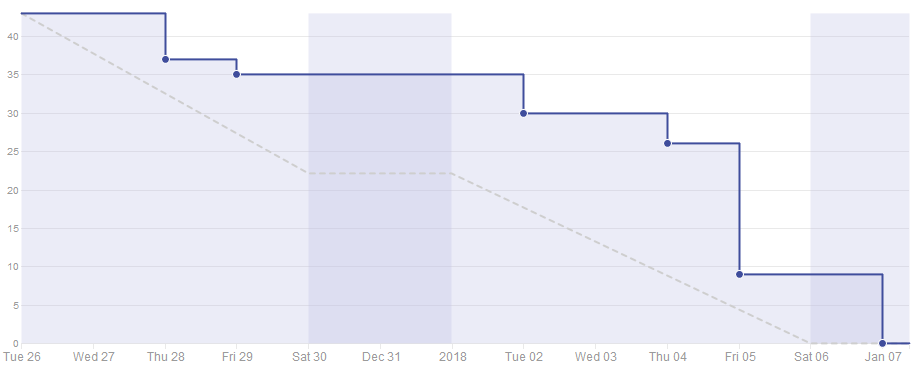
\includegraphics[width=0.95\textwidth]{Milestone14}
\caption{Burndown del sprint 13}
\label{fig:Milestone14}
\end{figure}

\subsection{Sprint 14 (08/01/18 - 14/01/18)}
Esta semana, se ha avanzado con la memoria, se han hecho algunas correcciones y mejoras:
\begin{itemize}
\item Corregir los notebook. Corregir los notebook para que funcionen correctamente, ya que al descargarlos de Github no encuentra bien las librerías.
\item Correcciones menores. Corregir fallos menores, entre ellos:
	\begin{itemize}
		\item En Rotation Forest utilizar el conjunto reducido según las clases (instance\_classes).
		\item En Random Oracles ver porque no funciona al dibujar la gráfica.
		\item En las clases ensemble modificar el base\_estimator.
	\end{itemize}
\item Memoria correcciones. Corregir las partes de la memoria y anexos, que me han dicho los tutores.
\item Comentar ensembles. Comentar los métodos ensembles, corregir los base, ya que estos no son ensembles.
\item Mejorar el cómo detectar si es o no Multi-Label. En vez de la comprobación que hago, utilizar el método \texttt{is\_multilabel}.
\item \texttt{predict\_proba} Random Oracles. Error encontrado en el \texttt{predict\_proba}, no devuelve los valores de forma correcta.
\end{itemize}

Esta semana se han cumplido todas las tareas, en la tarea de las correcciones mínimas he tenido que dedicar más tiempo del esperado.

En la figura~\ref{fig:Milestone15} se muestra el gráfico del Sprint 14.

\begin{figure}
\centering
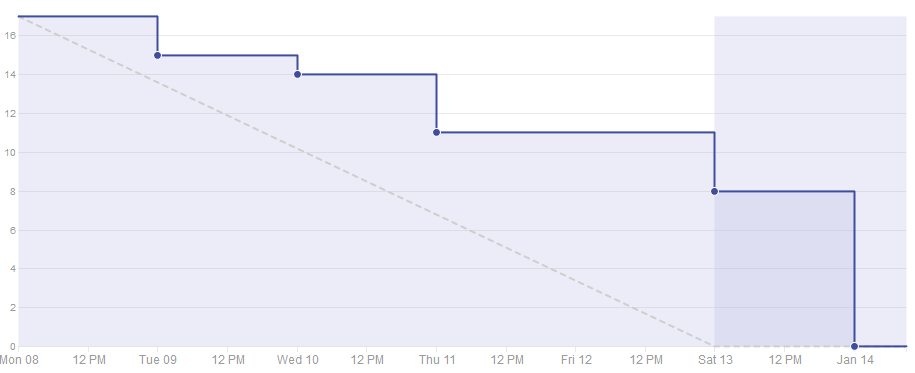
\includegraphics[width=0.95\textwidth]{Milestone15}
\caption{Burndown del sprint 14}
\label{fig:Milestone15}
\end{figure}

\subsection{Sprint 15 (16/01/18 - 22/01/18)}
Esta semana, se ha avanzado con la memoria y los anexos, y se han hecho algunas correcciones y mejoras:
\begin{itemize}
\item Diagrama de clases. Hacer los diagramas de clases que muestre las clases que hemos implementado.
\item Gráfica Random Oracle. La gráfica de RO no está bien, hay que buscar en que parte de nuestro algoritmo está el error.
\item Diagrama de secuencias. Hacer un diagrama de secuencias de uno de los notebook, en concreto el de los ensembles.
\item Memoria: Introducción. Mejorar la introducción, añadiendo cosas como que se ha seguido el estilo de Sklearn, y añadir que la minería de datos dentro tiene aprendizaje automático y dentro de este supervisado.
\item Añadir citas. Añadimos citas a los distintos algoritmos en el código.
\item Añadir ejemplos de uso. Añadir ejemplos de uso a los clasificadores, tomar como referencia el de \textbf{DecisionTreeClassifier}.
\item Hacer un notebook de las gráficas.A partir del python de las gráficas, crear un notebook en jupyter con ellas.
\item Notebook base classifiers. Pequeñas correciones, como todo en inglés o que falla un clasificador al dibujar el árbol.
\item Mejoras en los notebooks. Una misma cabecera para todos, poner un índice, comprobar que todos los notebooks funcionan correctamente.
\item Mejoras en el código. Algunos comentarios que no están correctos o faltan, mejorar la comprobación de cuando el conjunto de datos que nos pasan es Multi-Label. 
\item Árbol random oracles. Al intentar dibujar el árbol sale un error. El problema es que como este clasificador base tiene dos o más clasificadores(en función del número de oráculos), solo podemos dibujar un árbol.
\item Mejoras en conceptos teóricos. Mejoramos los conceptos teóricos de Scikit-Learn, Multi-Label y Ensembles.
\item Anexos: Añadir sprints. Añadir los sprints hasta el día de hoy.
\item Rellenar el README.md. 
\item Memoria: RO y RF. En conceptos teóricos documentar los ensembles Random Oracles y Rotation Forest.
\item Revisar la guía de estilo PEP8. Revisar la guía de estilos PEP8, para los notebooks.

\end{itemize}

Esta semana se han cumplido todas las tareas, y se han hecho en el tiempo estimado.

En la figura~\ref{fig:Milestone16} se muestra el gráfico del Sprint 15.

\begin{figure}
\centering
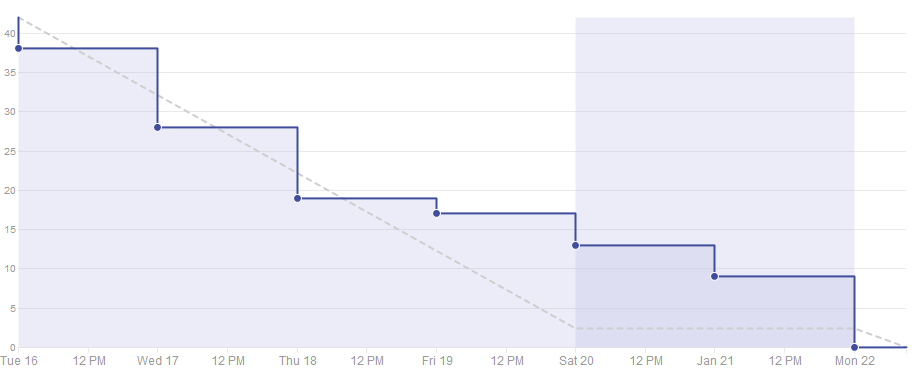
\includegraphics[width=0.95\textwidth]{Milestone16}
\caption{Burndown del sprint 15}
\label{fig:Milestone16}
\end{figure}

\subsection{Sprint 16 (23/01/18 - 30/01/18)}
Esta semana, se ha avanzado con la memoria y los anexos, se ha utilizado la herramienta SonarQube y se han hecho pruebas para probar los algoritmos:
\begin{itemize}
\item SonarQube. Utilizar la aplicación SonarQube para ver que no hay código duplicado.
\item Añadir técnicas y herramientas. Añadir nuevas técnicas y herramientas como por ejemplo Graphviz, Zenhub o Python.
\item Aspectos relevantes. Añadir aspectos relevantes como por ejemplo:
\begin{itemize}
	\item Leer documentación científica.
	\item Implementar algoritmos.
	\item Scikit-Learn.
	\item Generados notebooks.
\end{itemize}
\item Hacer pruebas. Hacemos pruebas para ver el correcto funcionamiento.
Las hacemos sobre \textbf{DecisionTreeClassifier} comparado con nuestros tres algoritmos mediante la validación cruzada.
\item Mejorar conceptos teóricos. Mejorar los conceptos teóricos de minería de datos, \textit{ensembles} y Multi-Label.
\item Manual del programador. Incluir en el Anexo de manual del programador: cómo he incluido el proyecto en SonarQube, la URL, y los comentarios (Porque no he seguido las recomendaciones de SonarQube).
\item Anexos: Diseño arquitectónico. Vamos acabar la parte de diseño del anexo realizando la parte de diseño arquitectónico, en la que se mostrará la estructura de nuestro proyecto.
\item Problemas en notebooks. En los notebooks de \textit{Graphics} y el de \textit{DT vs ensembles} corregir fallos.
\end{itemize}

Esta semana se han cumplido todas las tareas, aunque como el notebook en el que realizamos las pruebas había algún error, tuvimos que dedicar algo más de tiempo del estimado.

En la figura~\ref{fig:Milestone17} se muestra el gráfico del Sprint 16.

\begin{figure}
\centering
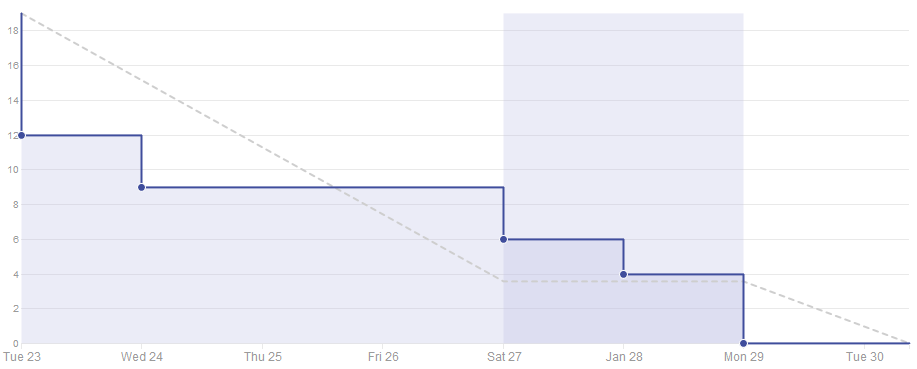
\includegraphics[width=0.95\textwidth]{Milestone17}
\caption{Burndown del sprint 16}
\label{fig:Milestone17}
\end{figure}

\section{Estudio de viabilidad}
En esta sección vamos a realizar un estudio de viabilidad económica de nuestro proyecto y su viabilidad legal, ya que son los dos aspectos mas relevantes.
\subsection{Viabilidad económica}
Se va a hacer un estudio de viabilidad económica del proyecto. Se van a analizar los gastos que hubiera supuesto, si fuese un proyecto real, para una empresa, en cuanto al tiempo requerido de programación e infraestructura.
\subsubsection{Costes de personal}
Este proyecto ha sido realizado por un programador que ha estado durante cuatro meses y medio trabajando en él.
Las hora que se han ido realizado han sido detalladas en la herramienta ZenHub podemos estimar que el proyecto consta de 366 Horas a 10 \euro~la hora:

\[10~{\mbox{\euro}} /\textsf{Hora}*385\textsf{Horas}=3850~{\mbox{\euro}}\]

Por otro lado también vamos a incluir las horas de reuniones semanales con nuestro equipo de proyecto, los tutores, este aspecto serian 18 horas extra en reuniones y otras 15 horas aproximadamente en consultas con ellos.
\[10~{\mbox{\euro}} /\textsf{Hora}*33\textsf{Horas}=330 ~{\mbox{\euro}} \]

A esta cuantía debemos añadirle el valor que se debería llevar la Seguridad Social que equivaldría a:
\begin{itemize}
\item 23,6\%: Por Seguridad Social.
\item 5,5\%: Por desempleo.
\item 0,6\%: Por formación profesional.
\item 0,2\%: Por Fogasa.
\item Total: 29,9\% 
\end{itemize}
Y esto equivale a: 
\[4180~{\mbox{\euro}}*0.299=1250~{\mbox{\euro}}\]

Estos porcentajes se han sacado se la Seguridad Social\footnote{\url{http://www.seg-social.es/Internet_1/Trabajadores/CotizacionRecaudaci10777/Regimenes/RegimenGeneraldelaS10957/TablasResumendebase9932/TiposdeCotizacion/index.htm}}
\subsubsection{Costes de material}
Como el software utilizado es libre no tenemos ningún coste de licencias. La parte de hardware he usado mi propio ordenador que tiene un valor de 650 \euro, se considera que un ordenador se amortiza en cinco años y como nosotros lo hemos usado cuatro meses y medio, el coste de hardware ha sido:
\[\frac{650~{\mbox{\euro}}}{(12\textsf{Meses}*5\textsf{Periodos})}*4.5\textsf{MesesDeUso}=49~{\mbox{\euro}}\]
\subsubsection{Costes totales}
Como costes totales sumaremos todos los anteriores, como se puede observar en la tabla \ref{tab:costes}.

\begin{table}[]
\centering
\caption{Tabla de los costes totales}
\label{tab:costes}
\rowcolors {2}{gray!35}{}
%\resizebox{0.5\textwidth}{!}{
\begin{tabular}{p{4cm} p{2cm}}
\toprule
Costes & Importe \\ \midrule
Personal         & 3\,850 \euro{}   \\ 
Seguridad Social & 1\,250 \euro{} \\ 
Material         & 49 \euro{}   \\ 
Totales             & 5\,149 \euro{} \\ \bottomrule
\end{tabular}
%}
\end{table}

\subsection{Viabilidad legal}
Se va hacer un análisis de las librerías que hemos usado en nuestro proyecto. Buscar los tipos de licencias que tienen cada uno, luego analizar, dependiendo de las compatibilidades, que tipos de licencia podemos aplicar nuestro proyecto y seleccionaremos la más restrictiva.

\begin{table}[]
	\centering
	\caption{Tabla de librerías y sus licencias}
	\label{tabla:Licencias}
	\rowcolors {2}{gray!35}{}
	\begin{tabular}{l l l l}
	\toprule
	Librería     & Versión & Descripción                                                     & Licencia                \\ 	\midrule                     \\ 	
	Numpy        & 1.13  & \begin{tabular}[c]{@{}l@{}}Procesamiento de arrays para\\ números, strings y objetos.\end{tabular} & BSD                     \\ 
	Scikit-Learn & 0.19.1  & \begin{tabular}[c]{@{}l@{}}Librería para minería de datos y análisis de datos.\end{tabular}	               & BSD                     \\
	Matplotlib   & 1.5.3   & \begin{tabular}[c]{@{}l@{}}Librería Python para mostrar\\ gráficos 2D.\end{tabular}                      & PSF-based               \\ 
	Graphviz     & 2.38    & \begin{tabular}[c]{@{}l@{}}Librería para visualizar árboles. 
\end{tabular}                      & MIT   \\
	Liac-arff    & 2.1.1   & \begin{tabular}[c]{@{}l@{}}Un módulo para leer y escribir\\ archivos arff en Python. \end{tabular}                      & MIT  
\\ \bottomrule
\end{tabular}
\end{table}


Aunque las licencias BSD y MIT son permisivas entre sí~\cite{wiki:BSD}, como la mayor parte del software utilizado es BSD, nuestro software llevará dicha licencia.


